\documentclass[14pt]{beamer}
\setbeamertemplate{itemize item}{$\bullet$}
\setbeamertemplate{navigation symbols}{}
\setbeamertemplate{mini frames}{}
\setbeamertemplate{section in toc}[sections numbered]
\setbeamertemplate{itemize items}[square]
\setbeamercolor*{item}{fg=gray}
\usecolortheme{dove}
\hypersetup{pdfpagemode=FullScreen}

\usepackage[yyyymmdd]{datetime}

% Define some accent colours:
\definecolor{DarkFern}{HTML}{407428}
\definecolor{DarkCharcoal}{HTML}{4D4944}
\colorlet{Fern}{DarkFern!85!white}
\colorlet{Charcoal}{DarkCharcoal!85!white} 
\colorlet{LightCharcoal}{Charcoal!50!white}
\colorlet{AlertColor}{orange!80!black}
\colorlet{DarkRed}{red!70!black}
\colorlet{DarkBlue}{blue!70!black}
\colorlet{DarkGreen}{green!70!black}
\definecolor{palecerulean}{rgb}{0.61, 0.77, 0.89}

% Use the colours:
\setbeamercolor{alerted text}{fg=palecerulean}
\setbeamercolor{title}{fg=blact}

% Create horizontal rule, header, and title page
\makeatletter
\def\vhrulefill#1{\leavevmode\leaders\hrule\@height#1\hfill \kern\z@}
\makeatother
\setbeamertemplate{frametitle}{\color{black}\bfseries\insertframetitle\par\vskip-6pt\color{palecerulean}\vhrulefill{1.75pt}}
\defbeamertemplate*{title page}{customized}[1][]
{
	{\begin{centering}
	\usebeamerfont{title}\bfseries\inserttitle\par\bigskip
	\usebeamerfont{subtitle}\insertsubtitle\par\vskip-3pt\color{palecerulean}\vhrulefill{1.75pt}\color{black}\\
	\bigskip
	\bigskip
	\usebeamerfont{author}\insertauthor\par\bigskip
	\usebeamerfont{institute}\insertinstitute\par
	\usebeamerfont{date}\insertdate\par
	\usebeamercolor[fg]{titlegraphic}\inserttitlegraphic
				\insertframetitle\par
	\smallskip\end{centering}}
}


\title{Qui devrait avoir un~mot~à~dire~?}
\subtitle{Le cas des bavures policières aux États-Unis}
\author{Anthony Kevins}
\institute{École de gouvernance\\
	Université d’Utrecht}
\date{\today}


\begin{document}

\begin{frame}
\titlepage
\end{frame}

\begin{frame}
	\frametitle{Des impacts disproportionnés}
	\begin{figure}
		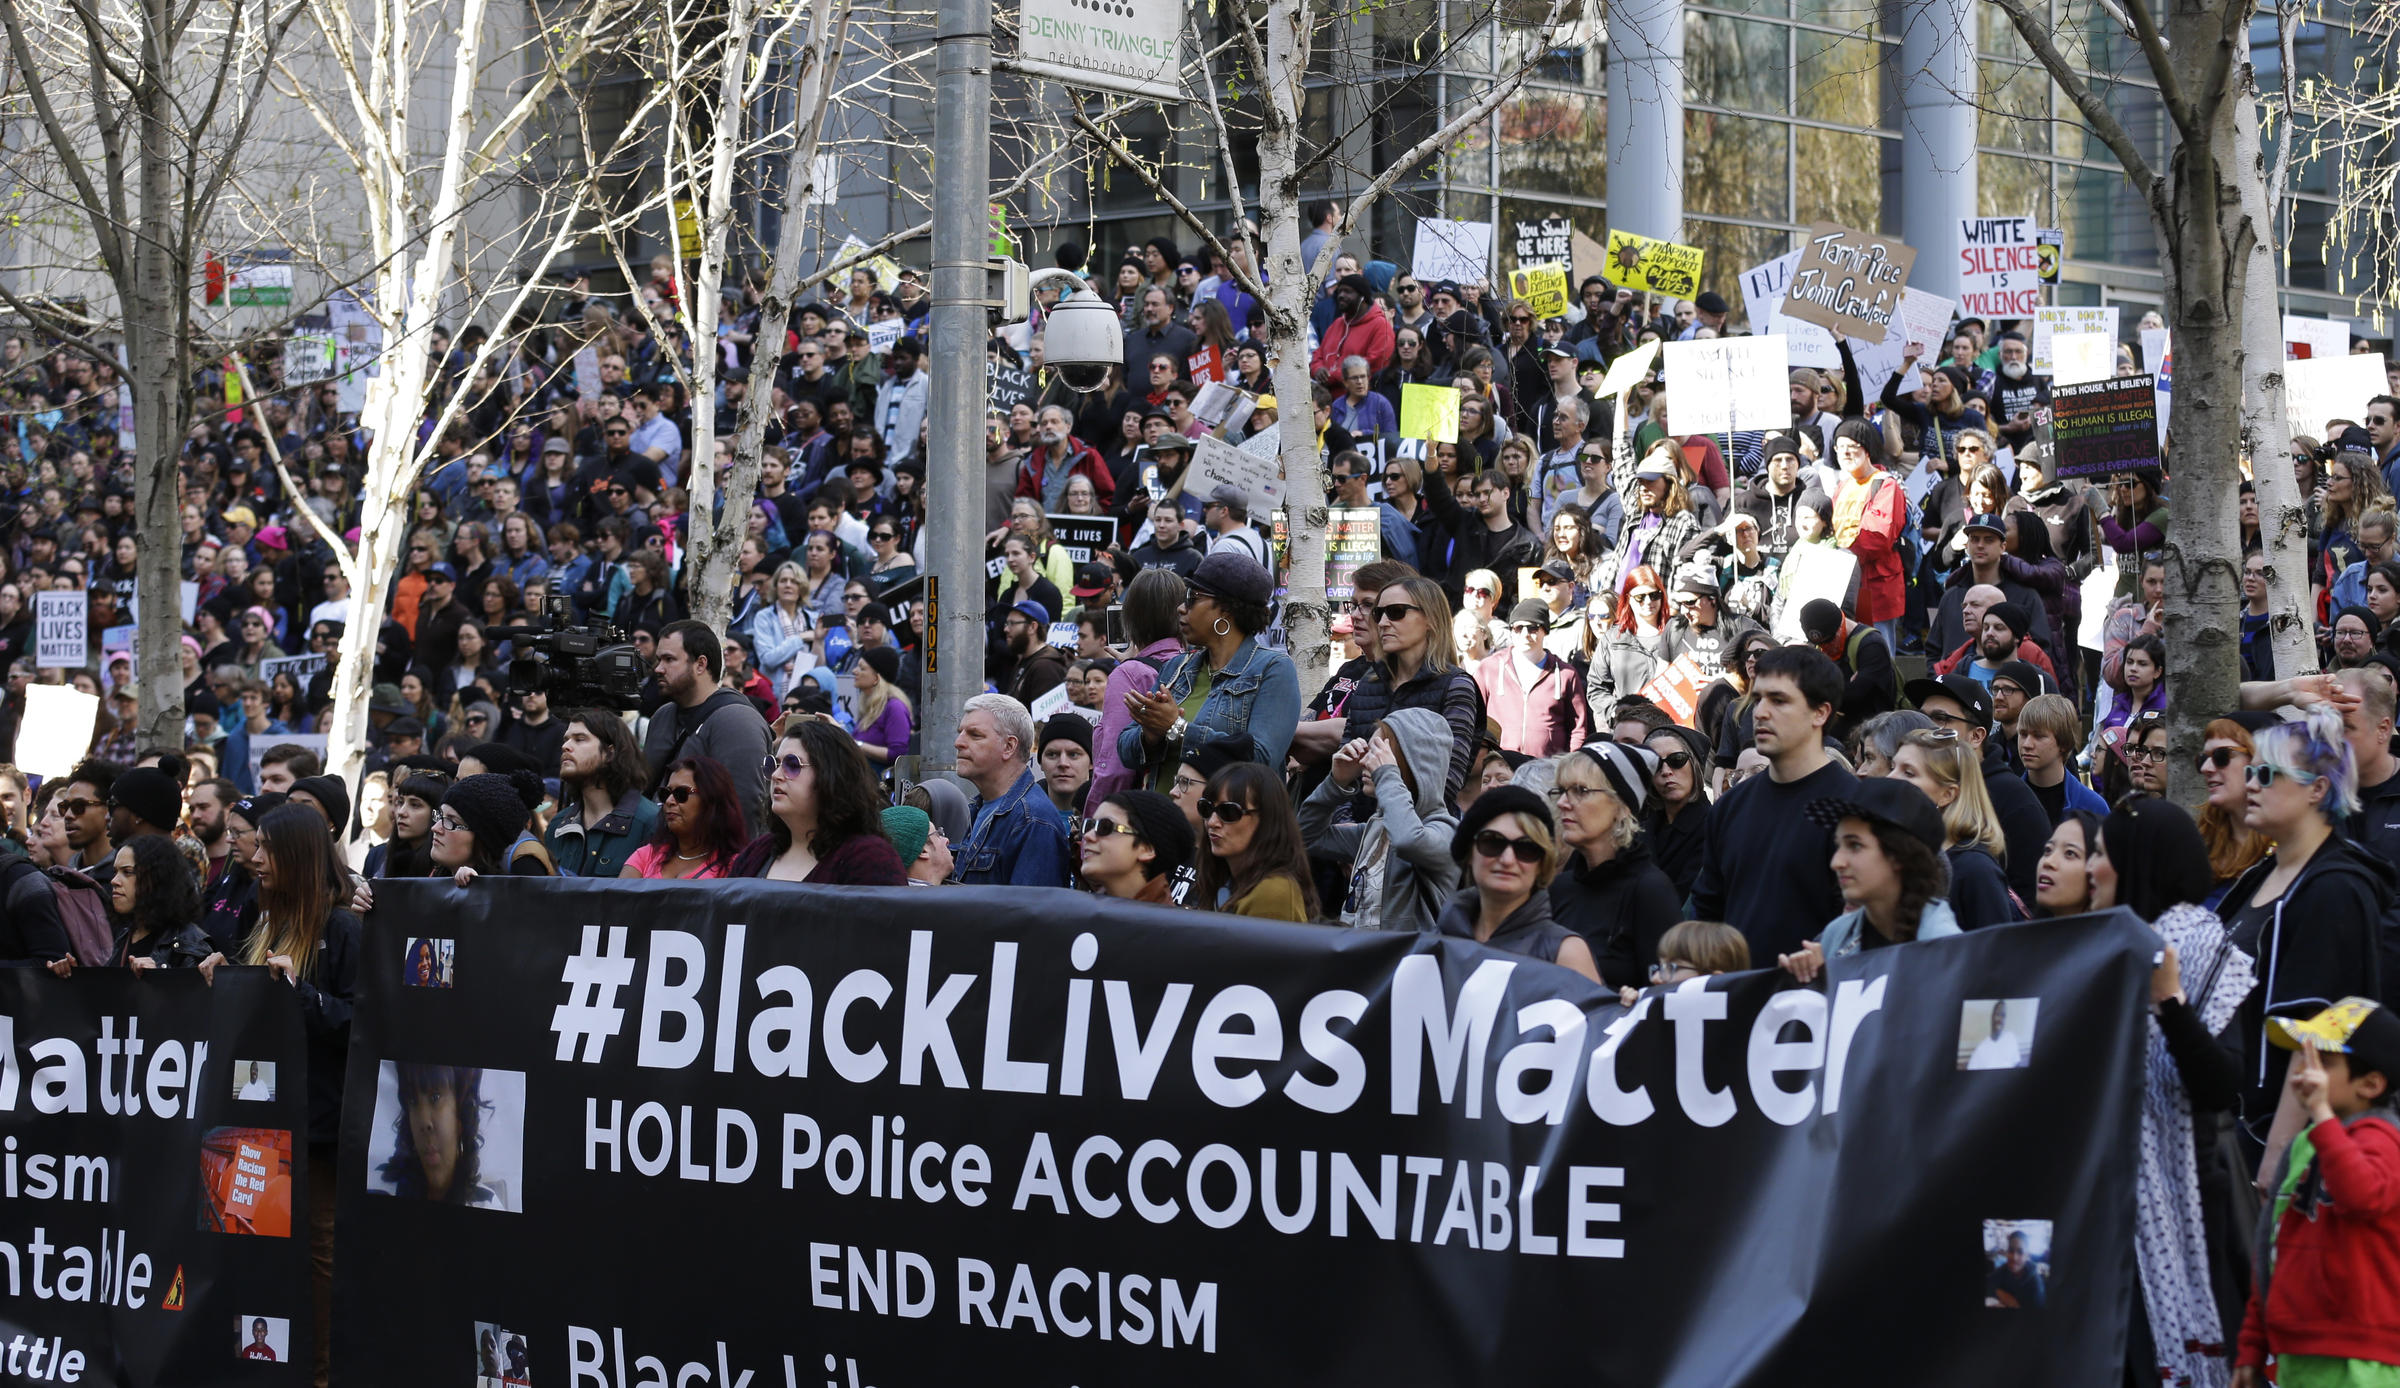
\includegraphics[scale=.4]{BLM}
	\end{figure}
	Aux États-Unis, les Afro-Américains constitue 13 \% de la population, mais 39 \% de victimes de bavures policières.\\
\end{frame}

\begin{frame}
\frametitle{Comment régler l'enjeu ?}
Une solution potentielle : 

\begin{itemize}
	\pause
	\item Mener des consultations auprès de la communauté Afro-Américain 
	\pause
	\item Reformuler les directives de la police à la lumière de ces discussions
\end{itemize}
\pause
\bigskip
Mais, dans les yeux des citoyens, est-il acceptable d'accorder une influence disproportionnelle à un groupe minoritaire ?
\end{frame}

\begin{frame}
\frametitle{Une solution démocratique ?}
Deux visions de l'opinion publique sur une telle proposition :
\begin{enumerate}
	\pause 
	\item Un engagement général en faveur de l'équité formelle
	\begin{itemize}
		\pause 
		\item Pour le public, la démocratie exige un traitement identique de chaque citoyen
		\pause
		\item Une vision soutenue par plusieurs études, mais trop catégorique ?
	\end{itemize}
	\pause 
	\item Un engagement conjoncturel en faveur de l'équité substantielle
	\begin{itemize}
		\pause 
		\item L'influence peut être inégale, mais les préférences dépendent des détails du cas 
		\pause 
		\item Plus probable, mais quels facteurs importent ?
	\end{itemize}
\end{enumerate}
\end{frame}

\begin{frame}
\frametitle{L'étude}
Expérience intégrée dans une enquête menée auprès de 2250 Américains :\\
\bigskip

\begin{itemize}
	\pause 
	\item Questions sur les Afro-Américains et la police  
	\pause 
	\item Courte description du problème 
	\pause 
	\item Un politicien propose une solution
	\begin{itemize}
		\pause 
		\item Le plan : consulter toute la population locale OU consulter la communauté afro-américaine locale
		\pause 
		\item La race du politicien : Blanc OU Noir 
		\pause 
		\item Le parti du politicien : Démocrate OU Républicain
	\end{itemize}
	\pause 
	\item Questions sur la proposition et le politicien
	\pause 
	\item Questions personnelles 
\end{itemize}
\end{frame}

\begin{frame}
	\frametitle{Resultats}
	\begin{figure}
		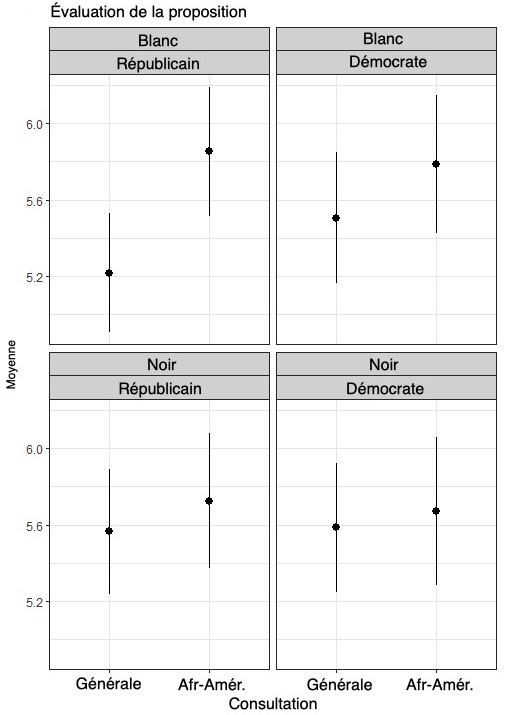
\includegraphics[scale=.3]{Fig1}
	\end{figure}
\end{frame}

\begin{frame}
	\frametitle{Resultats}
	\begin{figure}
		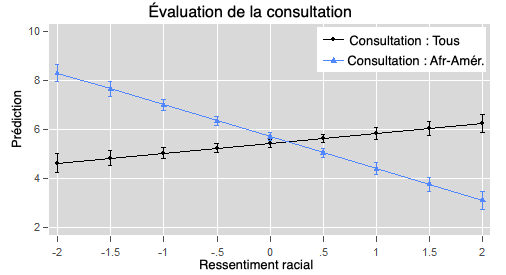
\includegraphics[scale=.6]{Fig3}
	\end{figure}
\end{frame}

\begin{frame}
	\frametitle{Conclusions}
	En décortiquant les réactions, on constate :
	\begin{itemize}
		\pause 
		\item variation significative générée par la forme de la consultation proposée ;
		\pause 
		\item aucun norme généralisée en faveur de l'équité formelle ;  
		\pause 
		\item les qualités du politicien n'ont eu qu'un impact limité ;
		\pause 
		\item et le ressentiment racial des sondés a joué un rôle crucial. 
	\end{itemize}
	
\end{frame}

\end{document}
